\subsubsection{Casos Bordes}

En esta secci\'on vamos a analizar ciertas familias de grafos en las cuales sabemos como se deber\'ia comportar el algoritmo exacto y que resultado tendr\'ia que devolver, para corroborar su correcto funcionamiento.
Esto no es una demostraci\'on de su correctitud, pero es una buena forma de ver si no se nos escapa la torutga.

Las familias que vamos a analizar son las siguientes:

\begin{itemize}
	\item Grafos con n nodos aisldos
	\item Grafos en forma de estrella
	\item Grafos que sean ciclos simples de n nodos
	\item Grafos completos con todos pesos 1 en sus aristas
\end{itemize}

$GRAFOS CON N NODOS AISLADOS$



Para esto generamos instancias de 0 a 100 nodos y no agergamos ninguna arista. Luego corrimos el algoritmo para k entre 2 y 50.\\
Pudimos verificar que el resultado de el algoritmo para cualquier grafo sin importar ni la cantidad de nodos, ni las particiones el resultado es siempre 0 como peso de la suma de las aristas intrapartici\'on lo cual es efectivamente cierto pues no existen aristas.\\

Corroboramos que el algoritmo exacto funciona correctamente para este tipo de instancias.

$GRAFOS ESTRELLA$

Para esto con el generador de instancias seleccionamos un nodo de forma aleatoria y lo conectamos al resto de los nodos.\\
Luego corrimos el algoritmo y nuevamente verificamos que se para cualquier cantidad de nodos y cualquier cantidad de particiones el peso total de la sumatoria de sus aristas es igual a 0.
Es razonable pues al nodo central se lo puede ubicar en alguna particion y al resto en cualquier otra, con lo cual no hay aristas intraparticion.

$CICLOS SIMPLES (C_n)$

Generamos grafos que eran ciclos de n elementos. Y esperabamos que tambien nos de 0 la sumatoria de las aristas sin importar la cantidad de nodos ni las particiones. Pero nos olvidamos que los ciclos simples de longitud impar no eran bipartitos. Con lo cual para cualquier grafo que sea un ciclo de longitud impar si corro el algoritmo para encontrar una 2-particion m\'inima esta nunca va a ser 0.

Pudimos corroborar que para todos los grafos que sean circuitos simples para cualquier k mayor o igual a 3 su k-PMP es 0. Y para todos los que sean circuitos simples de longitud impar y para una 2-particion la sumatoria de sus aristas intraparticion es igual a la menor de las aristas

$K_n CON PESOS 1$

Con el generador de isntancias creamos grafos completos de n elementos con todos sus pesos en 1.

Pudimos verificar que el peso de las sumatoria de sus aristas intraparticion es:

\bc
	$k * (((n  div  k) * ((n  div  k) - 1)/2)) + (n  mod  k) * (n  div  k)$
\ec

B\'asicamente esto es as\'i pues en cada partici\'on voy a tener como m\'inimo n div k nodos que se conectan todos entre todos por ser un grafo completo. Con lo cual esa partici\'on va a aportar ((n div k) * ((n div k) - 1)/2) al peso total pues todas sus aristas intraparticion pesan 1. Luego tengo k particiones y por ultimo el resto de dividir a n por k son los nodos que me restan que los tengo que ubicar en alguna particion y estos se conectan con el resto de los nodos de esa particion.


\subsubsection{Rendimiento}

Para el análisis de rendimiento, corrimos el algoritmo variando la cantidad de particiones de 2 a 7, 100 instancias aleatoreas para cada n entre 5 y 20 de las cuales sacamos el promedio de tiempos, para las tres familias de grafos con el 15\%, 50\% y 100\% de sus aristas, tanto con el algoritmo sin podas y con podas.


\bc
\begin{tabular}{l c}
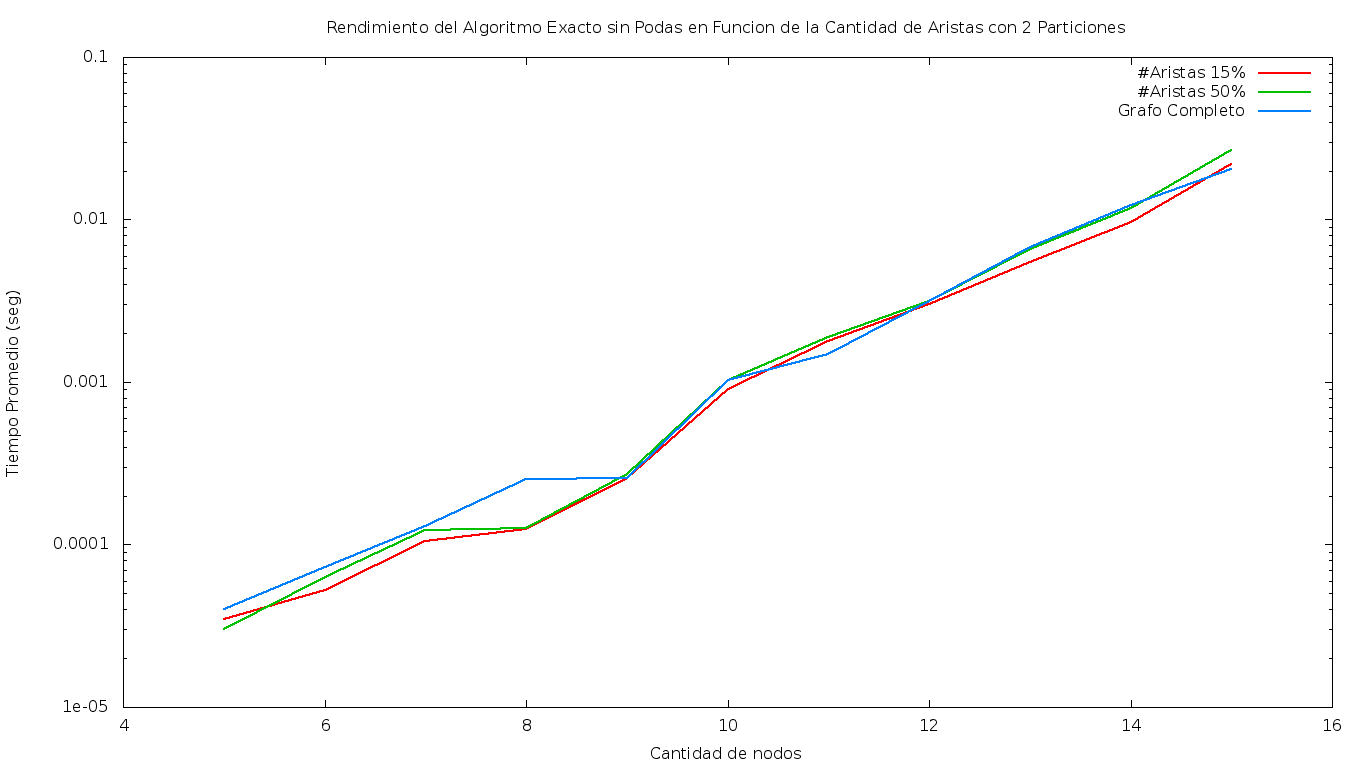
\includegraphics[scale=0.16]{finales/rendimientoExactoSinPoda2Particiones.png}
&
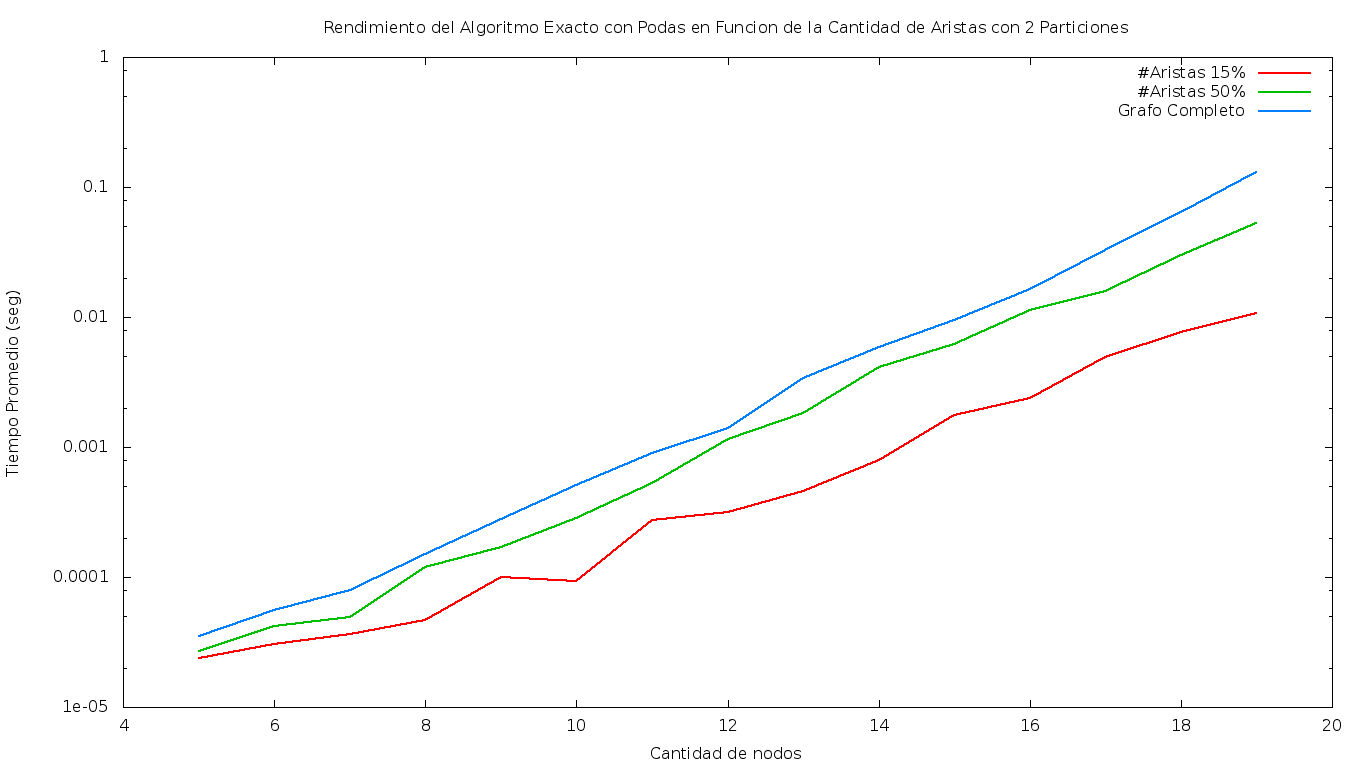
\includegraphics[scale=0.16]{finales/rendimientoExactoConPoda2Particiones.png}
\end{tabular}
\ec

\bc
\begin{tabular}{l c}
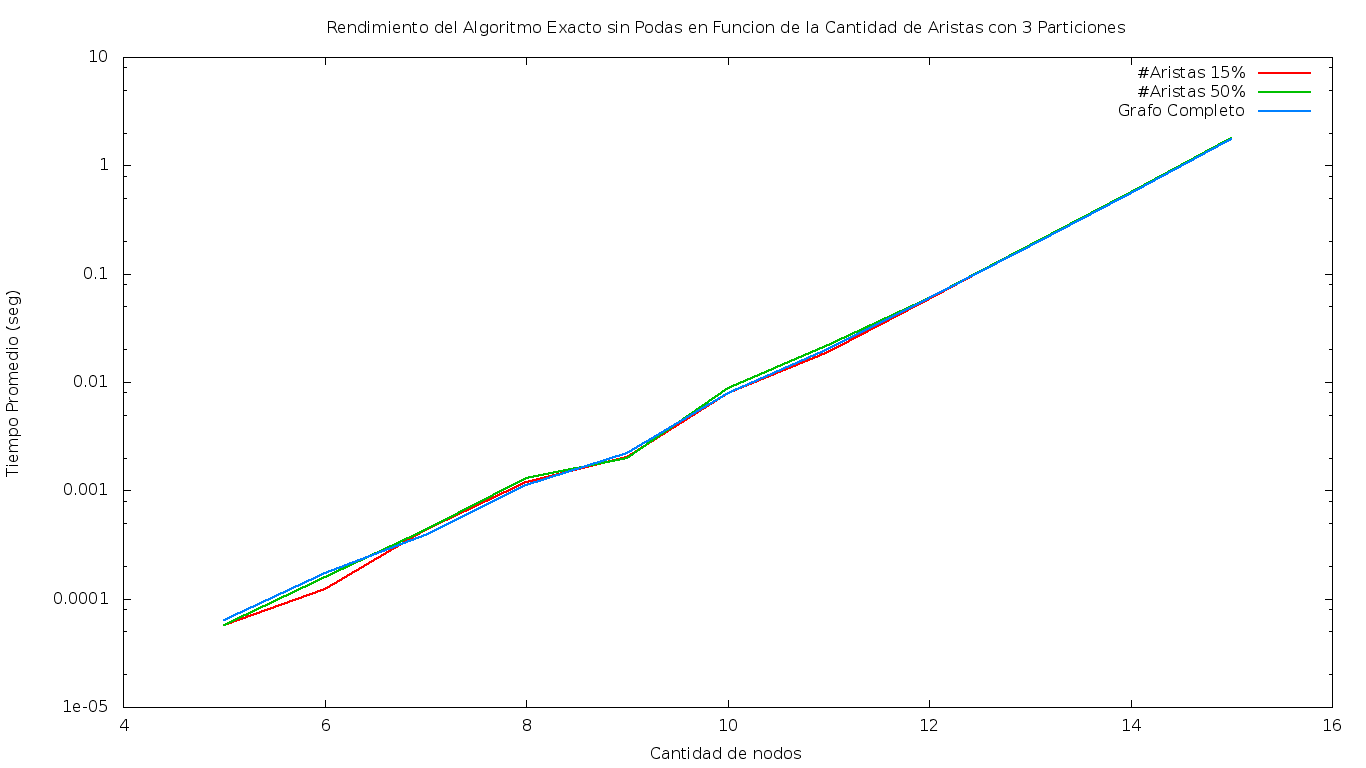
\includegraphics[scale=0.16]{finales/rendimientoExactoSinPoda3Particiones.png}
&
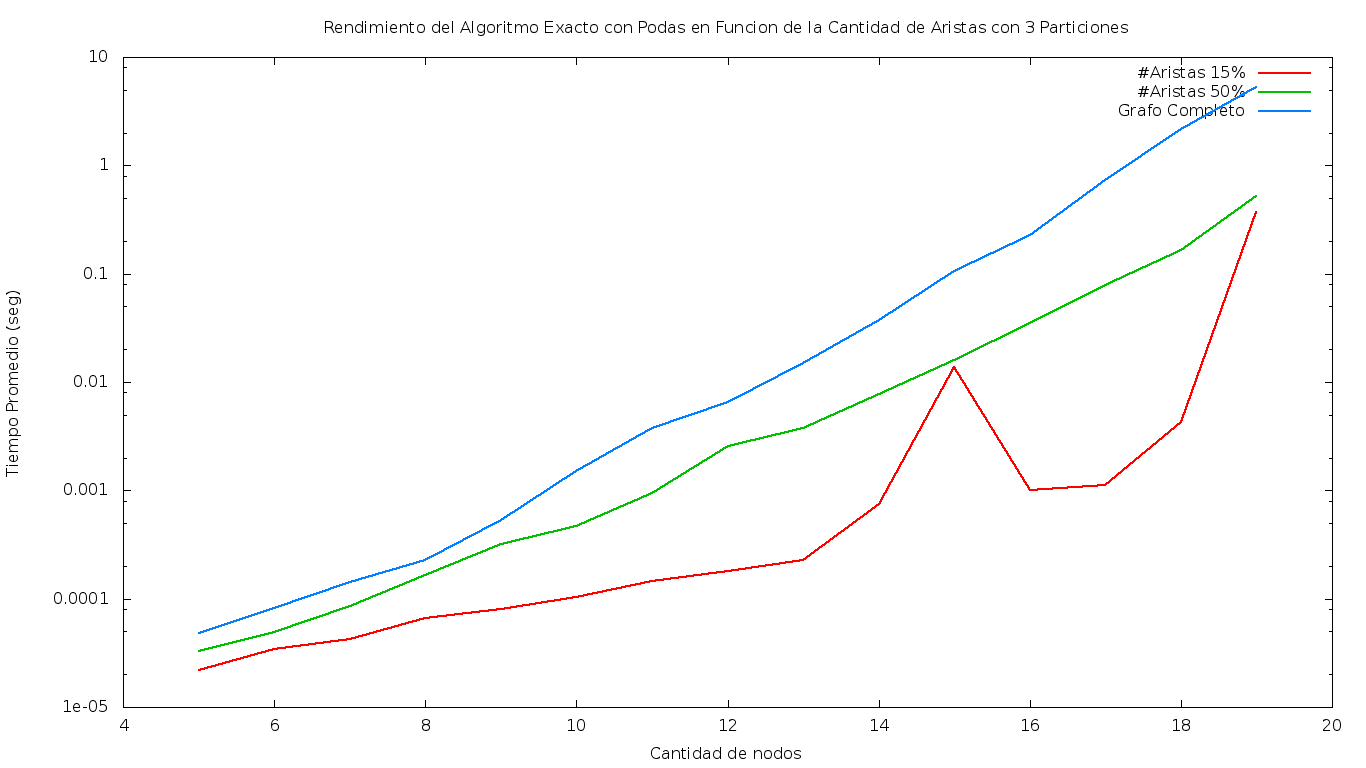
\includegraphics[scale=0.16]{finales/rendimientoExactoConPoda3Particiones.png}
\end{tabular}
\ec

\bc
\begin{tabular}{l c}
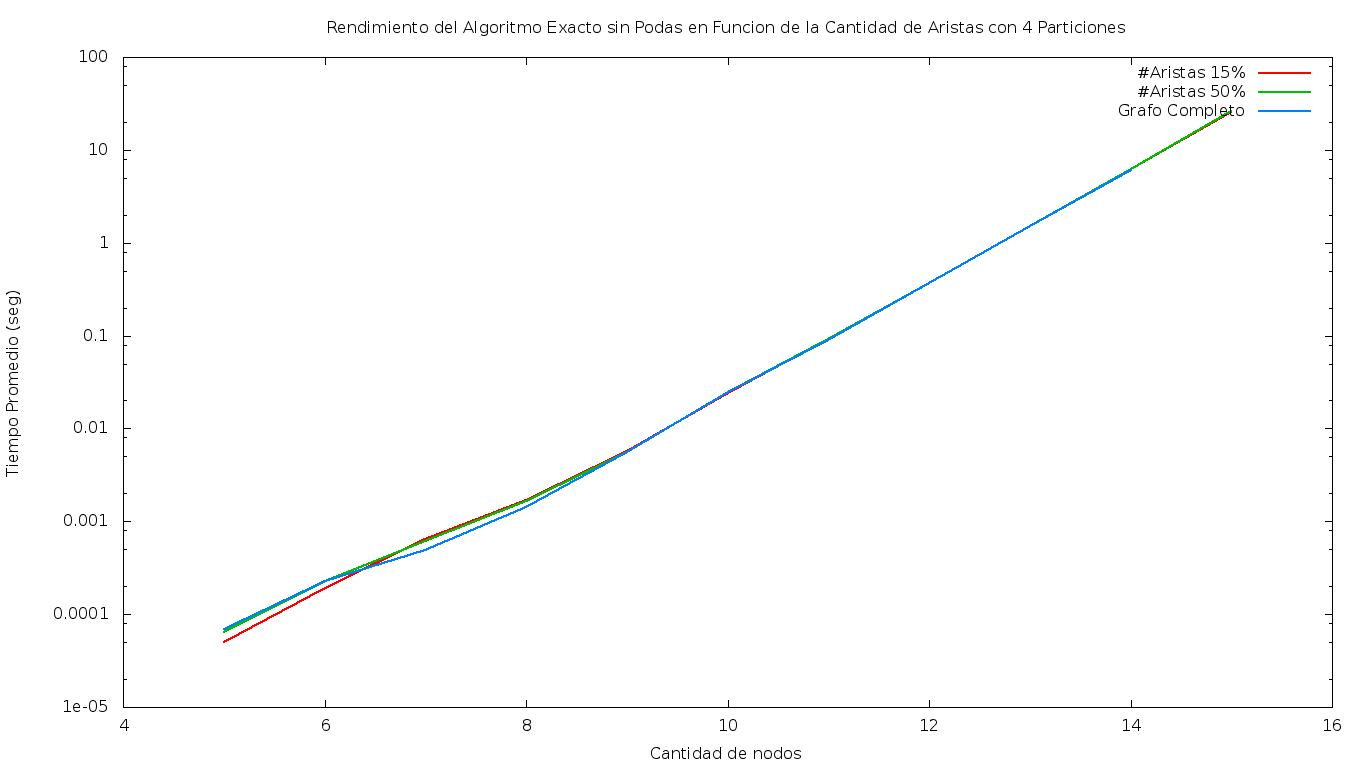
\includegraphics[scale=0.16]{finales/rendimientoExactoSinPoda4Particiones.png}
&
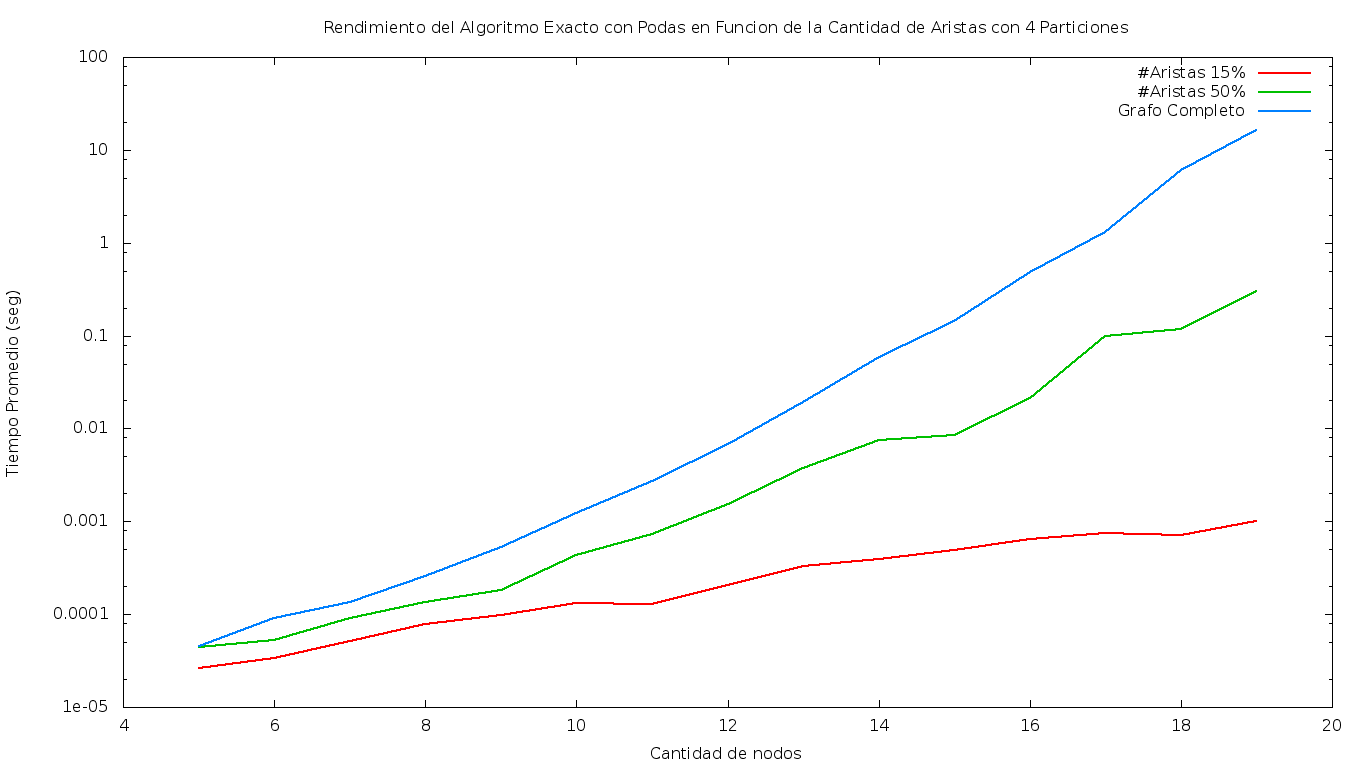
\includegraphics[scale=0.16]{finales/rendimientoExactoConPoda4Particiones.png}
\end{tabular}
\ec

\bc
\begin{tabular}{l c}
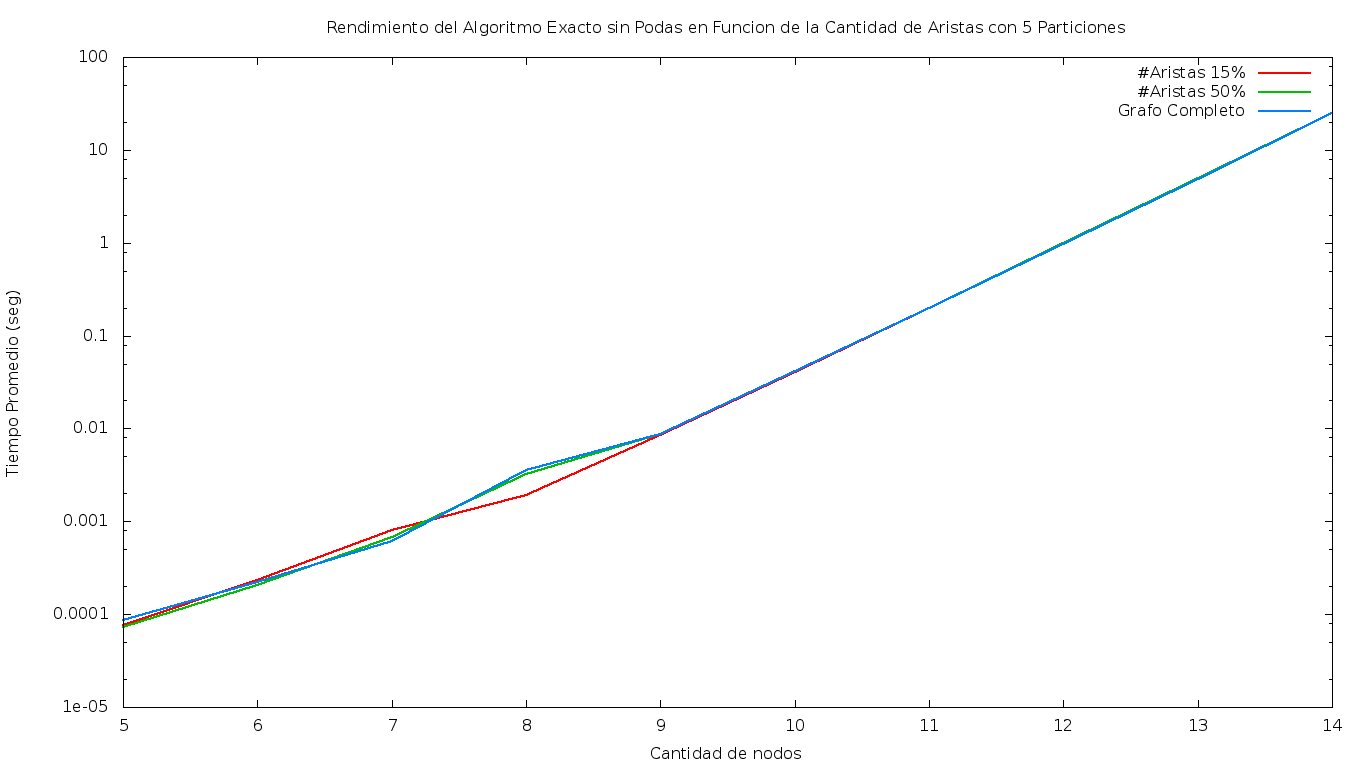
\includegraphics[scale=0.16]{finales/rendimientoExactoSinPoda5Particiones.png}
&
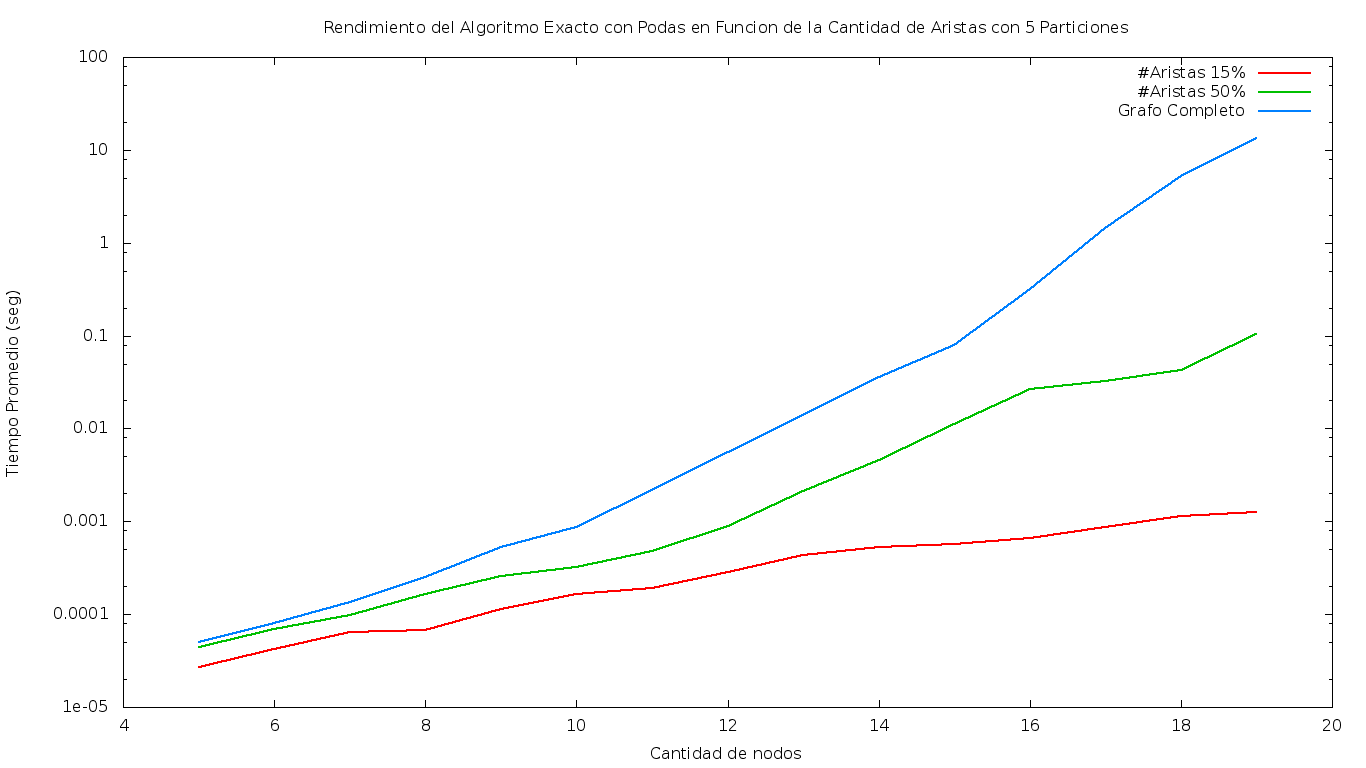
\includegraphics[scale=0.16]{finales/rendimientoExactoConPoda5Particiones.png}
\end{tabular}
\ec

\bc
\begin{tabular}{l c}
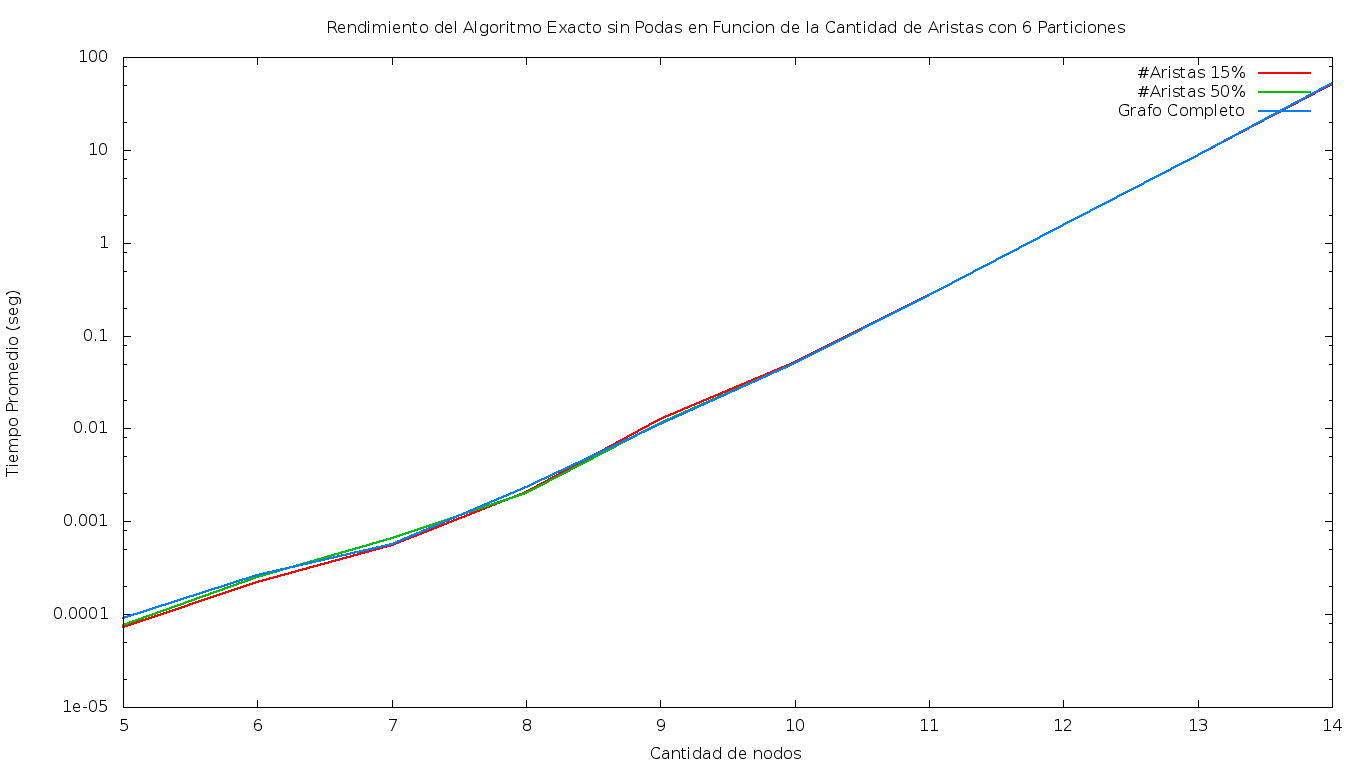
\includegraphics[scale=0.16]{finales/rendimientoExactoSinPoda6Particiones.png}
&
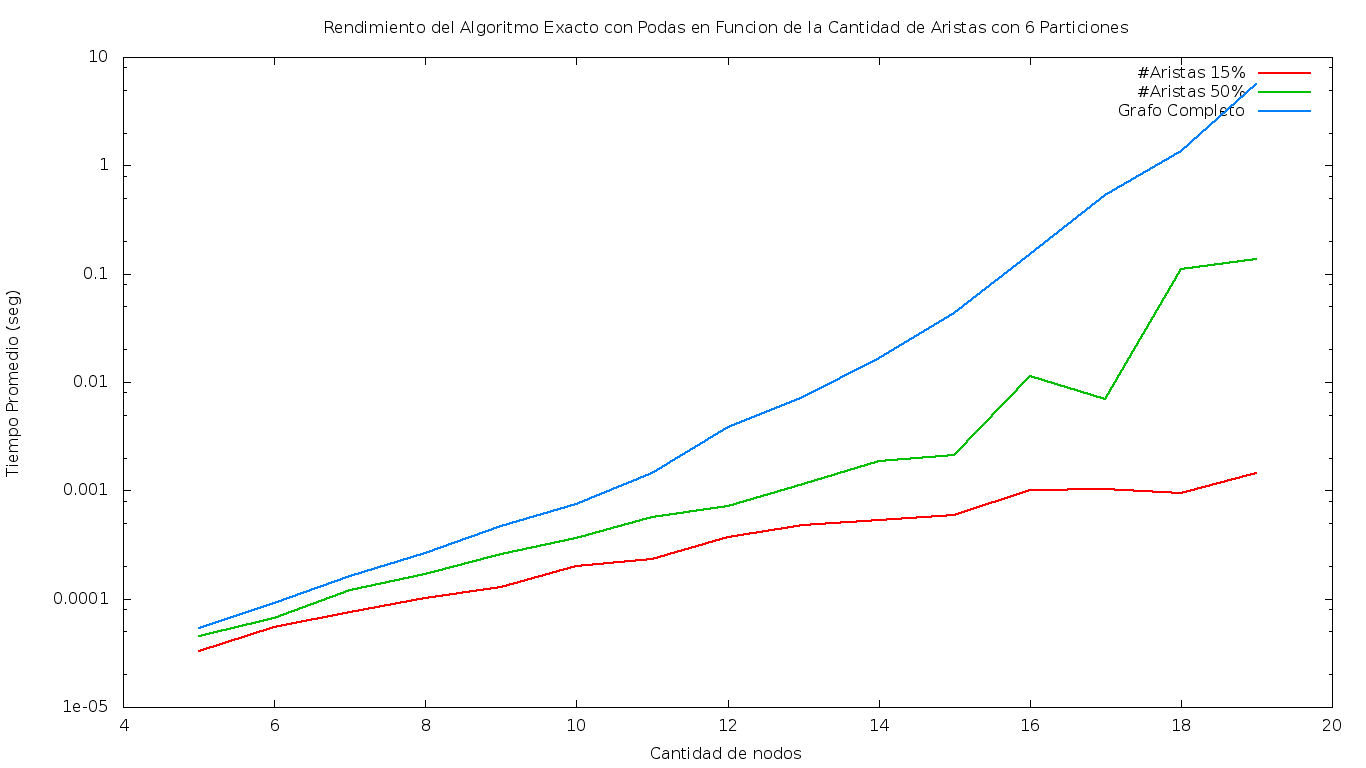
\includegraphics[scale=0.16]{finales/rendimientoExactoConPoda6Particiones.png}
\end{tabular}
\ec

\bc
\begin{tabular}{l c}
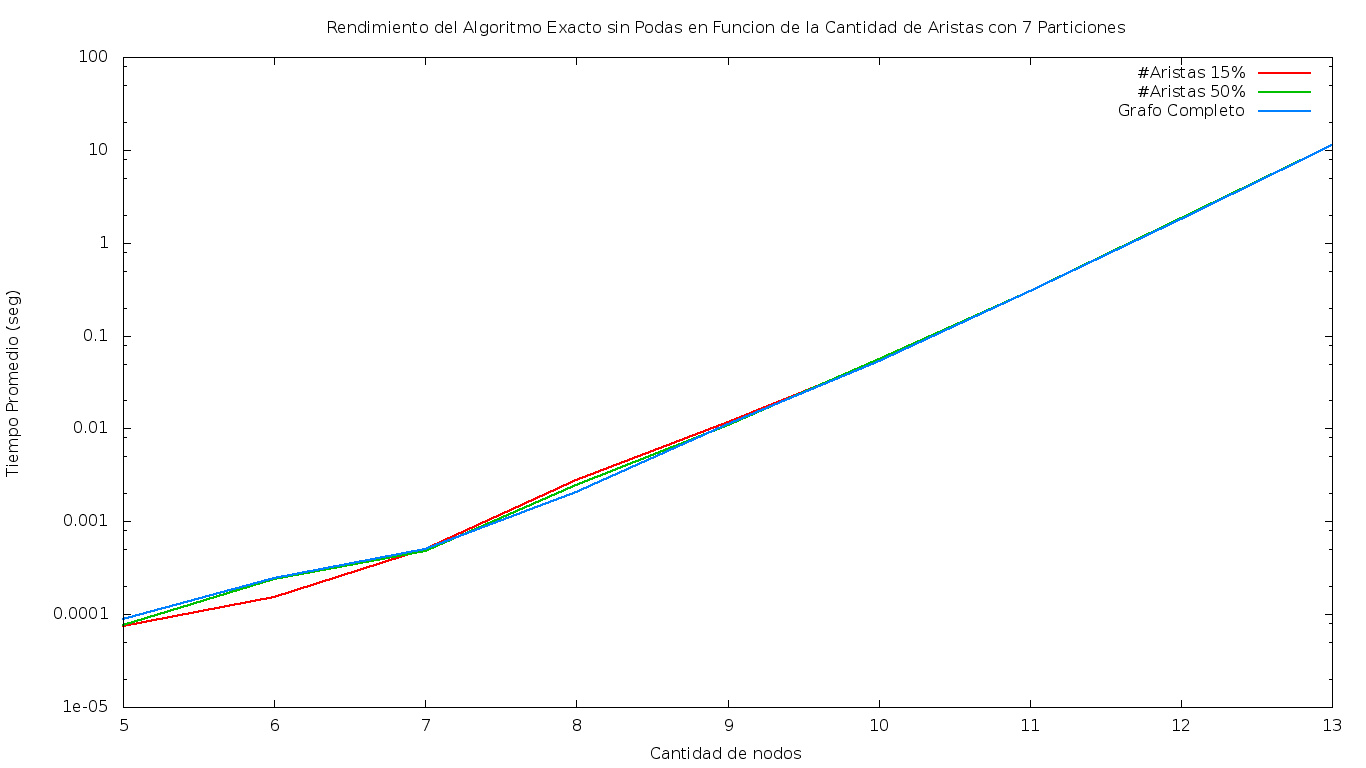
\includegraphics[scale=0.16]{finales/rendimientoExactoSinPoda7Particiones.png}
&
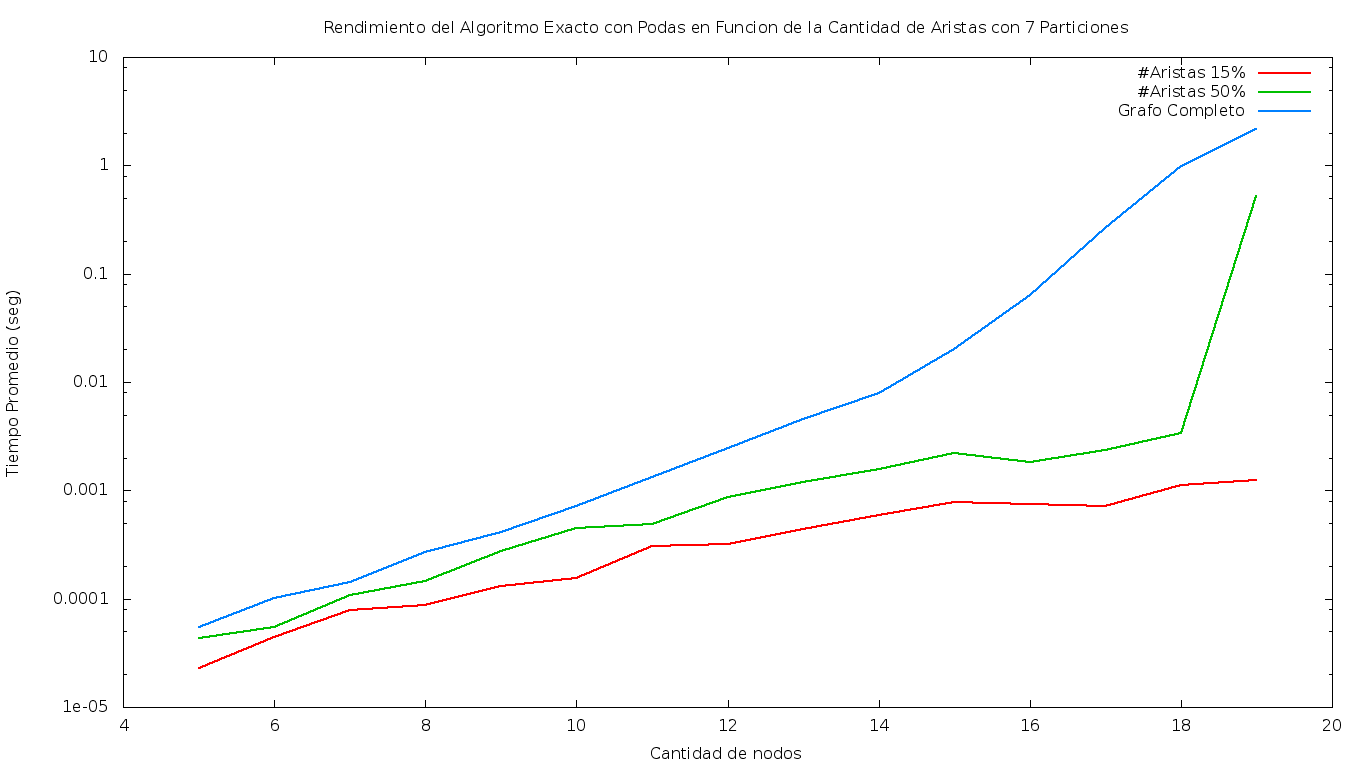
\includegraphics[scale=0.16]{finales/rendimientoExactoConPoda7Particiones.png}
\end{tabular}
\ec

